% pdflatex new.tex %
\documentclass{article}

\usepackage{graphicx}

\title{C++ Parallel application for Traveling Salesman Problem resolution using genetic algorithm}
\author{Berti Stefano}
\date{\today}

\begin{document}
    \thispagestyle{plain}
    % Titles %
    \begin{center}
        \Large
        \textbf{C++ Parallel application for Traveling Salesman Problem resolution using genetic algorithm}

        \vspace{0.4cm}
        \large Parallel and Distributed System: Paradigms and Models
        \\2019 / 2020

        \vspace{0.4cm}
        \textbf{Berti Stefano}

        \vspace{0.9cm}
        \textbf{Abstract}
    \end{center}
    % Abstract %
    The aim of this project is to implement a genetic algorithm for the resolution of the Traveling Salesman Problem and to parallelize it with two different mechanism:
    \begin{itemize}
	\item C++ standard threads and mutex
	\item Fastflow library
    \end{itemize}
    \section{Problem description}\label{sec:s1}

        Genetic algorithms mimic natural evolution. In order to do that, we need a population of chromosomes, a way to assign an affinity score to each chromosome and transform it into a probability to select which elements of the population will surivive (and so will reproduce), how those chromosomes reproduce and how mutation can occour. We also have 2 fixed probabilities for crossover and mutation to happen.
	\begin{itemize}
	    \item \textbf{City}: the city is made by two vectors of integers for the 2 coordinates (node i has coordinates (x[i], y[i]), each x has range [0, 640], each y has range [0, 480]). It also has an adjacent matrix (vector of vector of bool) for the possible path of dimensions \#nodes*\#nodes, which is automatically optimized to use just 1 bit for each element.
	    \item \textbf{Population}: it is a matrix (vector of vector), where each row contains a sequence of number, and each number represent a node
	    \item \textbf{Affinity}: for each element x is the probability that x will be selected for reproduction, and is calculated as the inverse of the path length, normalized w.r.t. all other elements in order to obtain a proper probability
	    \item \textbf{Reproduction}: 2 paths A and B can create a new path C by generating 2 random numbers i and j and putting the subsequence B[i, j] in A. If checking the adjacent matrix we find out that C is not a feasible path, we try again until C is feasible.
	    \item \textbf{Mutation}: a mutation occour with a certain probability to every new generated chromosome, and it is a random shuffle of two position in the generated C path. The probability that a mutation does not occour is 0.9, which is a good trade-off (too high leads to casuality, too low leads to no evolution). If checking the adjacent matrix we find out that C is not a feasible path, we try again until C is feasible.
	\end{itemize}
	To calculate the length of each path, I use a random generated city, where for each node number we have the relative coordinates, picked up randomly in a window of size 640x480. It is possible to plot the city, the connections among the nodes (blue dotted line) and the best solution found untill the current interation at runtime by compiling with \textbf{make compile-graph}, this is available only for the sequential version and has huge impact on the performance, but shows the correctness of the algorithm. This algorithm is not guaranteed to find the best solution of TSP, which is a NP problem, but can find a good starting point for successive improvements.

    \begin{figure}
        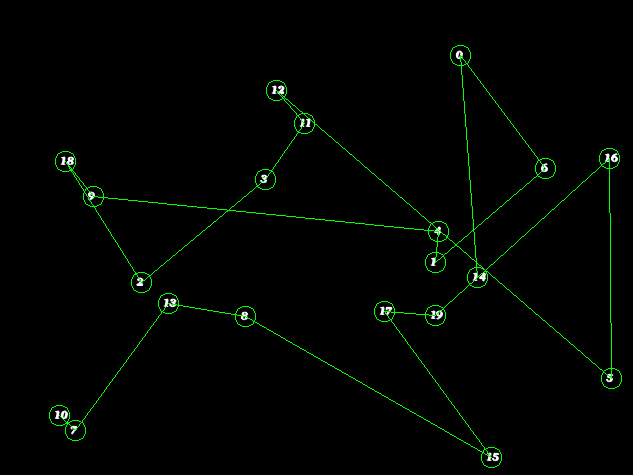
\includegraphics[width=\linewidth, height=8cm]{img/init.png}
        \caption{Initial problem with 20 nodes}
        \label{fig:init}
    \end{figure}
    \begin{figure}
        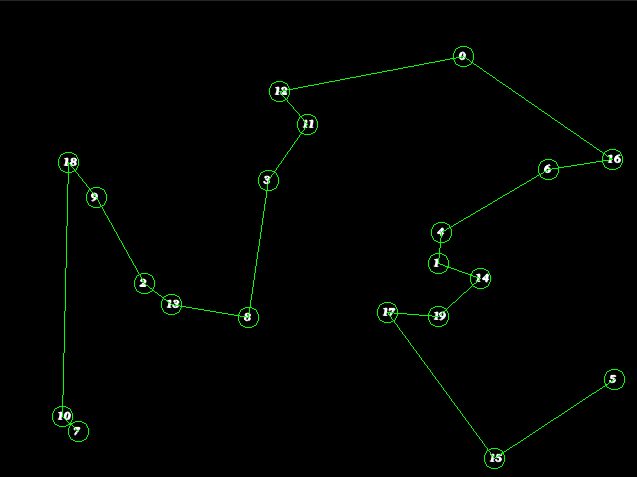
\includegraphics[width=\linewidth, height=8cm]{img/sol.png}
        \caption{Solution found after some iterations}
        \label{fig:sol}
    \end{figure}

    \section{A first approach}\label{sec:s2}
	The first approach that I though was to use the fact that we can divide each iteration in two phases, and each phase is parallelizable with a map. It was a pipeline with feedback composed by a map-reduce to calculate the affinity of each path by inverting the length, a reduce phase to compute the sum and to normalize each affinity in order to obtain proper probabilities and another map for the reproduction stage. Each worker had its own chunk of the population/affinities to compute, and the fastflow version was implemented with a parallelforreduce to compute the length of each path and to reduce on the sum, and another parallelfor to compute the new population.
    \begin{figure}
        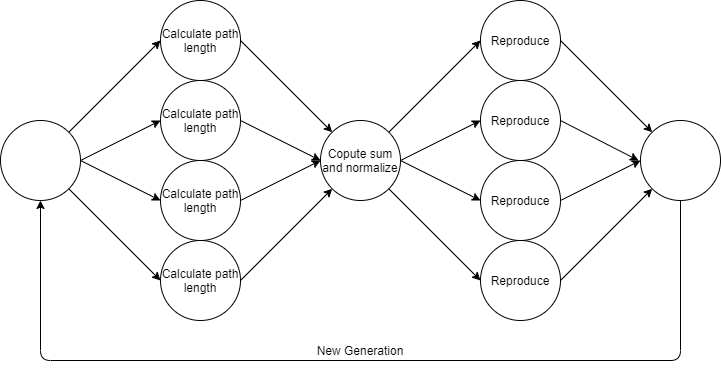
\includegraphics[width=\linewidth]{img/first.png}
        \caption{The first approach}
        \label{fig:first}
    \end{figure}
    This apporach ideally reduce the completion time by a factor of nw, but we need to have a barrier between the two phases and this leads to a lower speedup, because I needed to have proper probabilities for the second stage to be executed. The good of this apporach is that we have just one population with always the same size, independently by the number of workers, and the result shouldn't change too much w.r.t. the number of workers. But we can think to a different solution, which drives us to the \textbf{normal form}: when the population is big, the probabilities are all small and not very different because the path lengths don't differ too much, if I assume to have more than one independent populations, I will not make the same computation as before because I won't be considering anymore the possibility of crossover among each pair of chromosomes of the population, but I will get rid of the synchronization among workers, increasing performances and decreasing the completion time.

    \section{The second approach}\label{sec:s3}
	This approach is a simple farm over the task \textbf{evolve}, which is a composition of the two stages \textbf{calculate affinities} and \textbf{reproduce}. This composition is also known as\textbf{normal form}, and ensures the best performances with the lowest number of resources. In this way, the tasks are stateless, because we don't need to reduce on the state sum.
Considering that, provided enough iterations i, the scheduler and the gatherer times are negligible (the emitter just have to pass the parameters to the workers, and the gatherer just have to find the best solution over the nw solutions returned by the nw workers), the completion times is

	\centerline{$i*T_{w}/nw$}

    So, by increasing the number of workers, I expect to see a linear speedup. My machine has 5 cores, so I also expect to have the \textbf{knee} at 5 workers. The heaviest data structure is the \textbf{population} one, which has dimension 0.08MB (4 byte(int) * 20 * 1000), while affinities has size 0.008MB (8byte(double) * 1000) and city as a very small size around 320byte (8byte(double) * 2 * 20 and 20*20 bit for the adjacent matrix). My cpu has 3 caches L1, L2 and L3 of size respectively 9MB, 1.5MB and 350KB, so data easily fits the L3 cache and I don't expect a superlinear speedup.
    Anyway, I implemented the pick\_candidate function to cost O(n) in the worst case, where n is the population size, because it generates a random float and decreases this number with the probabilities one after the other untill it becomes negative, and then select the candidate as the number of iterations needed. This could generate a superlinear speedup, because increasing the number of workers, we are not reducing only the number of chromosomes that each worker has to generate, but also the time needed to generate each of them!

    \begin{figure}
        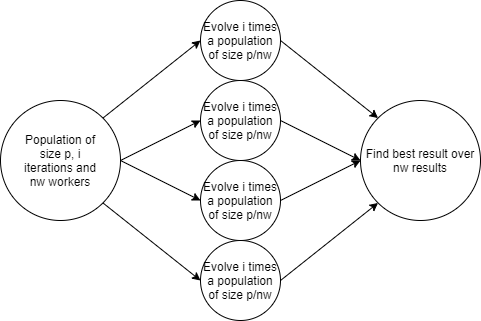
\includegraphics[width=\linewidth, height=8cm]{img/second.png}
        \caption{Second and final approach}
        \label{fig:second}
    \end{figure}


        \begin{table}[h!]
            \begin{center}
                \caption{Expected service time, real service time, gap between the two  and gap percentage w.r.t. real time for local randomized solution with 20 nodes, 10000 size of population and 1000 iterations (time in microseconds). My machine has 5 cores.}
                \label{tab:table1}
                \begin{tabular}{c|c|c|c|c}
                    \textbf{nw} & \textbf{T(nw)} & \textbf{(T(1)/nw)} & \textbf{gap} & \textbf{T(nw)/gap}\\
                    \hline
                        1 & 23334944 & 2341742 & 0 & 0\%\\
                        2 & 11828148 & 11667472 & 160676 & 1.3\%\\
			3 & 7937058 & 7778314 & 158743 & 2\%\\
			4 & 6065433 & 5833736 & 231697 & 3.8\%\\
			5 & 5055524 & 4666988 & 388536 & 7.6\%\\
			6 & 4975386 & 3889157 & 1086229 & 21\%\\
			7 & 5210023 & 3333563 & 1876460 & 36\%\\
                \end{tabular}
            \end{center}
        \end{table}


    \begin{figure}
        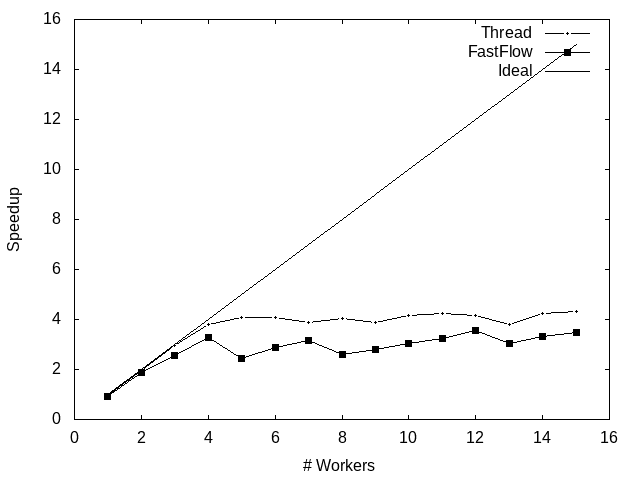
\includegraphics[width=\linewidth, height=8cm]{img/local_speedup.png}
        \caption{Local speed obtained with 20 nodes, 1000 chromosomes, 1000 iterations and 5 cores}
        \label{fig:locals}
    \end{figure}

    \begin{figure}
        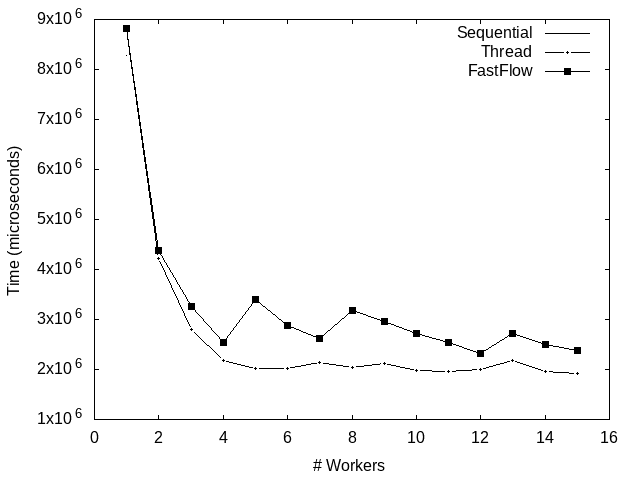
\includegraphics[width=\linewidth, height=8cm]{img/local_time.png}
        \caption{Local time obtained with 20 nodes, 1000 chromosomes and 1000 iterations and 5 cores}
        \label{fig:localt}
    \end{figure}

    \begin{figure}
        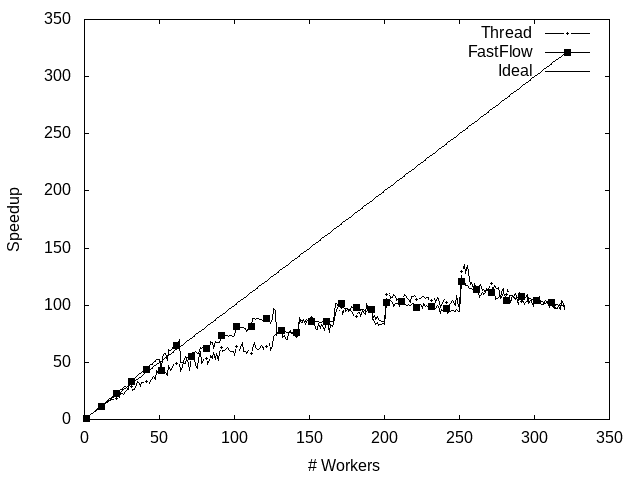
\includegraphics[width=\linewidth, height=8cm]{img/remote_speedup.png}
        \caption{Remote speedup obtained in phi19 machine, with 20 nodes, 1000 chromosomes, 1000 iterations and 256 cores}
        \label{fig:remotes}
    \end{figure}

    \section{Performance discussion}
	As we can see from the plots, in both the local and remote machine we have the knee in the expected point: at 5 in the local speedup because my machine has 5 cores and at 256 in the remote machine because it has 256 cores. The gap between the real speedup and the ideal one can be motivated by overheads, so the time needed to generate each thread (which becomes not negligible when nw gets higher) and the time to join them and to get the best results over the nw ones. The thread version is faster w.r.t. the FastFlow one because uses standard mechanisms of c++, which has less overheads w.r.t. the FastFlow library, even if the computation model is exactly the same.

    \section{Difficulties}
	At a certain point, I had a bottleneck in the remote machine that doesn't allow me to have a speedup higher than 3. I investigated this problem for days to find out that my bottleneck was caused by the \textbf{rand()} function. This, together with the pick candidate, made my development and my analysis a lot more difficult. To overcome this issue, i create the MyRandom class, which sets up just one time for worker the 3 differents uniform distribution that I use in the program, which are [0, n\_nodes)(int), [0, pop\_size)(int) and [0, 1](double).

    \section{Other improvements}
	I always compile my code with the -O3 flag in order to make other optimizations, like vectorization, which occour in various places: when we push work in the farm of FastFlow, in the main loop of the Evolution node of FastFlow (basic block), the affinities normalization, in the main loop of the thread (basic block), in the normalization of the sequential part, in the loop that starts the thread, int the loop that generates the population. Vectorization cannot happens in the main loop, because we need an \textbf{if} statement to check if the path just generated is the best untill now. I tried to parallelize other part of the code, for example the random inizialization of the city and of the population, but I didn't get any improvements, so I removed it.

    \section{Conclusions}
	I experimented first to preserve the flow of the algorithm with the usage of synchronization between stages and shared vector (that could also raise false sharing issues), then I decided to generate more smaller flows of execution of the algorithm in order to get the best one at the end of the computations. If we want to see which is the best path found from the workers at runtime, we have to be careful at the state access pattern, where the state is made by the best length and the best path. In the thread version, we can overcome this issue with the usage of a mutex around the block which controls and possibly sets the best state w.r.t. the new one, but then the maximum speedup reached would have been the ratio between Tw/Ta, where Ta is the time needed to access the state.

\end{document}
